% !TEX root = thesis.tex

\chapter{Object- and Region-Specific Retrieval}
\label{ch:8}
In the manual analysis of images, investigators often focus on particular objects in the scene, specifically those that are interesting or anomalous, rather than considering the image as a whole. This suggests an object-centric approach to automated methods for image matching. Figure~\ref{fig:wholeImVsObjectCentric} demonstrates the difference between a standard image based search that considers whole images with our proposed object-centric approach, where the investigator highlights a specific object in the image, and the search returns images containing similar looking objects. In Figure~\ref{fig:wholeImage}, the original search approach finds images with similar furniture configurations and color profiles. In the object-centric approach in Figure~\ref{fig:objectCentric}, the investigator highlighted the yellow lamp, and the search returns other images that contain similar lamps, regardless of the other content in the room. This proposed object-specific approach is not supported by existing approaches to image based search.

\begin{figure}
    \centering
    \begin{subfigure}[b]{3.2in}
        \begin{subfigure}[b]{1.05in}
            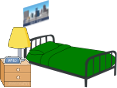
\includegraphics[height=.77in]{figures/chapter8/cartoonQueries/wholeIm1.png}
        \end{subfigure}
        \unskip \vrule
        \begin{subfigure}[b]{2.1in}
            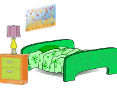
\includegraphics[height=.77in]{figures/chapter8/cartoonQueries/wholeIm2.png}
            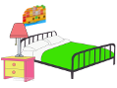
\includegraphics[height=.77in]{figures/chapter8/cartoonQueries/wholeIm3.png}
        \end{subfigure}
        \caption{Whole Image Search}
        \label{fig:wholeImage}
    \end{subfigure}
    \begin{subfigure}[b]{3.2in}
        \begin{subfigure}[b]{1.05in}
            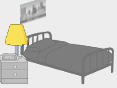
\includegraphics[height=.77in]{figures/chapter8/cartoonQueries/justLamp1.png}
        \end{subfigure}
        \unskip \vrule
        \begin{subfigure}[b]{2.1in}
            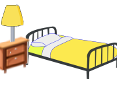
\includegraphics[height=.77in]{figures/chapter8/cartoonQueries/justLamp2.png}
            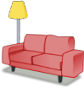
\includegraphics[height=.77in]{figures/chapter8/cartoonQueries/justLamp3.png}
        \end{subfigure}
        \caption{Object-centric Image Search}
        \label{fig:objectCentric}
    \end{subfigure}
    \caption[Whole image search vs. object-centric search]{(a) In a typical image search based on the whole image the results are the images that look most similar to the entire image (e.g., similar color profiles and furniture in the same configuration). (b) In our object-centric image search, the input is a selected object of interest, and the results are images that contain objects that are most similar to the query object (e.g., images with yellow lamps).}
    \label{fig:wholeImVsObjectCentric}
\end{figure}



\begin{figure*}
    \centering
    \setlength\tabcolsep{2pt}
    \renewcommand{\arraystretch}{2}
    \begin{subfigure}[b]{\textwidth}
    \begin{tabular}{lc|cc|cc|cc}
       \multicolumn{2}{c|}{Query Image} & \multicolumn{6}{|c}{Top Matches}  \\
        \hline
        Whole Image &
        \raisebox{-.5\height}{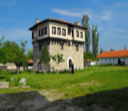
\includegraphics[height=\tableImHeight]{figures/chapter7/objSimilarity/landmarks/orig/query.png}} & 
        \raisebox{-.5\height}{\fcolorbox{green}{green}{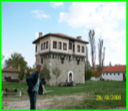
\includegraphics[height=\tableImHeight]{figures/chapter7/objSimilarity/landmarks/orig/1_im.png}}} & 
        \raisebox{-.5\height}{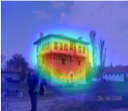
\includegraphics[height=\tableImHeight]{figures/chapter7/objSimilarity/landmarks/orig/1_hm.png}} &
        \raisebox{-.5\height}{\fcolorbox{red}{red}{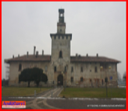
\includegraphics[height=\tableImHeight]{figures/chapter7/objSimilarity/landmarks/orig/2_im.png}}} & 
        \raisebox{-.5\height}{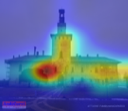
\includegraphics[height=\tableImHeight]{figures/chapter7/objSimilarity/landmarks/orig/2_hm.png}} &
        \raisebox{-.5\height}{\fcolorbox{red}{red}{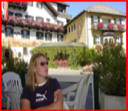
\includegraphics[height=\tableImHeight]{figures/chapter7/objSimilarity/landmarks/orig/3_im.png}}} & 
        \raisebox{-.5\height}{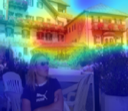
\includegraphics[height=\tableImHeight]{figures/chapter7/objSimilarity/landmarks/orig/3_hm.png}} 
        \\
        Region 1 &
        \raisebox{-.5\height}{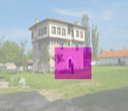
\includegraphics[height=\tableImHeight]{figures/chapter7/objSimilarity/landmarks/1/query.png}} & 
        \raisebox{-.5\height}{\fcolorbox{green}{green}{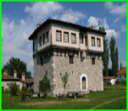
\includegraphics[height=\tableImHeight]{figures/chapter7/objSimilarity/landmarks/1/1_im.png}}} & 
        \raisebox{-.5\height}{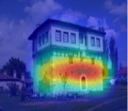
\includegraphics[height=\tableImHeight]{figures/chapter7/objSimilarity/landmarks/1/1_hm.png}} & 
        \raisebox{-.5\height}{\fcolorbox{red}{red}{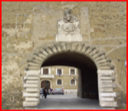
\includegraphics[height=\tableImHeight]{figures/chapter7/objSimilarity/landmarks/1/2_im.png}}} & 
        \raisebox{-.5\height}{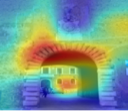
\includegraphics[height=\tableImHeight]{figures/chapter7/objSimilarity/landmarks/1/2_hm.png}} & 
        \raisebox{-.5\height}{\fcolorbox{red}{red}{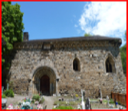
\includegraphics[height=\tableImHeight]{figures/chapter7/objSimilarity/landmarks/1/3_im.png}}} & 
        \raisebox{-.5\height}{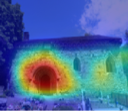
\includegraphics[height=\tableImHeight]{figures/chapter7/objSimilarity/landmarks/1/3_hm.png}} 
        \\
        Region 2 &
        \raisebox{-.5\height}{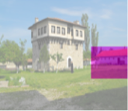
\includegraphics[height=\tableImHeight]{figures/chapter7/objSimilarity/landmarks/2/query.png}} & 
        \raisebox{-.5\height}{\fcolorbox{red}{red}{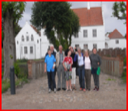
\includegraphics[height=\tableImHeight]{figures/chapter7/objSimilarity/landmarks/2/1_im.png}}} & 
        \raisebox{-.5\height}{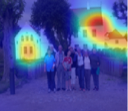
\includegraphics[height=\tableImHeight]{figures/chapter7/objSimilarity/landmarks/2/1_hm.png}} & 
        \raisebox{-.5\height}{\fcolorbox{red}{red}{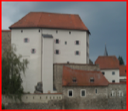
\includegraphics[height=\tableImHeight]{figures/chapter7/objSimilarity/landmarks/2/2_im.png}}} & 
        \raisebox{-.5\height}{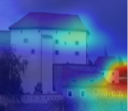
\includegraphics[height=\tableImHeight]{figures/chapter7/objSimilarity/landmarks/2/2_hm.png}} & 
        \raisebox{-.5\height}{\fcolorbox{red}{red}{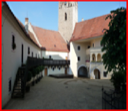
\includegraphics[height=\tableImHeight]{figures/chapter7/objSimilarity/landmarks/2/3_im.png}}} & 
        \raisebox{-.5\height}{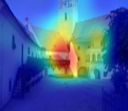
\includegraphics[height=\tableImHeight]{figures/chapter7/objSimilarity/landmarks/2/3_hm.png}} 
        \end{tabular}
    \caption{Google Landmarks}
    \end{subfigure}
    \begin{subfigure}[b]{\textwidth}
        \begin{tabular}{lc|cc|cc|cc}
        Whole Image &
        \raisebox{-.5\height}{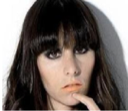
\includegraphics[height=\tableImHeight]{figures/chapter7/objSimilarity/faces/orig/query.png}} & 
        \raisebox{-.5\height}{\fcolorbox{green}{green}{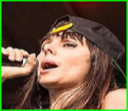
\includegraphics[height=\tableImHeight]{figures/chapter7/objSimilarity/faces/orig/1_im.png}}} & 
        \raisebox{-.5\height}{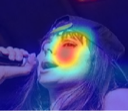
\includegraphics[height=\tableImHeight]{figures/chapter7/objSimilarity/faces/orig/1_hm.png}} & 
        \raisebox{-.5\height}{\fcolorbox{red}{red}{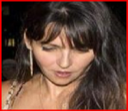
\includegraphics[height=\tableImHeight]{figures/chapter7/objSimilarity/faces/orig/2_im.png}}} & 
        \raisebox{-.5\height}{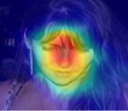
\includegraphics[height=\tableImHeight]{figures/chapter7/objSimilarity/faces/orig/2_hm.png}} & 
        \raisebox{-.5\height}{\fcolorbox{red}{red}{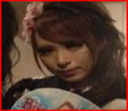
\includegraphics[height=\tableImHeight]{figures/chapter7/objSimilarity/faces/orig/3_im.png}}} & 
        \raisebox{-.5\height}{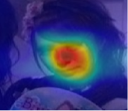
\includegraphics[height=\tableImHeight]{figures/chapter7/objSimilarity/faces/orig/3_hm.png}} 
        \\
        Region 1 &
        \raisebox{-.5\height}{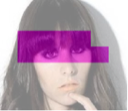
\includegraphics[height=\tableImHeight]{figures/chapter7/objSimilarity/faces/1/query.png}} & 
        \raisebox{-.5\height}{\fcolorbox{red}{red}{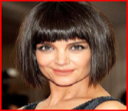
\includegraphics[height=\tableImHeight]{figures/chapter7/objSimilarity/faces/1/1_im.png}}} & 
        \raisebox{-.5\height}{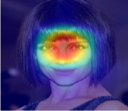
\includegraphics[height=\tableImHeight]{figures/chapter7/objSimilarity/faces/1/1_hm.png}} & 
        \raisebox{-.5\height}{\fcolorbox{green}{green}{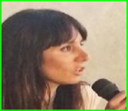
\includegraphics[height=\tableImHeight]{figures/chapter7/objSimilarity/faces/1/2_im.png}}} & 
        \raisebox{-.5\height}{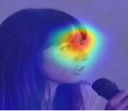
\includegraphics[height=\tableImHeight]{figures/chapter7/objSimilarity/faces/1/2_hm.png}} & 
        \raisebox{-.5\height}{\fcolorbox{red}{red}{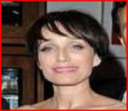
\includegraphics[height=\tableImHeight]{figures/chapter7/objSimilarity/faces/1/3_im.png}}} & 
        \raisebox{-.5\height}{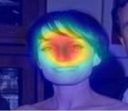
\includegraphics[height=\tableImHeight]{figures/chapter7/objSimilarity/faces/1/3_hm.png}} 
        \\
        Region 2 &
        \raisebox{-.5\height}{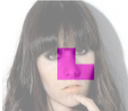
\includegraphics[height=\tableImHeight]{figures/chapter7/objSimilarity/faces/2/query.png}} & 
        \raisebox{-.5\height}{\fcolorbox{red}{red}{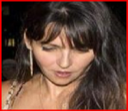
\includegraphics[height=\tableImHeight]{figures/chapter7/objSimilarity/faces/2/1_im.png}}} & 
        \raisebox{-.5\height}{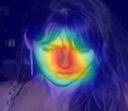
\includegraphics[height=\tableImHeight]{figures/chapter7/objSimilarity/faces/2/1_hm.png}} & 
        \raisebox{-.5\height}{\fcolorbox{red}{red}{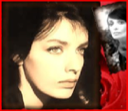
\includegraphics[height=\tableImHeight]{figures/chapter7/objSimilarity/faces/2/2_im.png}}} & 
        \raisebox{-.5\height}{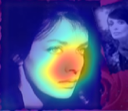
\includegraphics[height=\tableImHeight]{figures/chapter7/objSimilarity/faces/2/2_hm.png}} & 
        \raisebox{-.5\height}{\fcolorbox{red}{red}{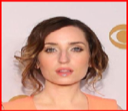
\includegraphics[height=\tableImHeight]{figures/chapter7/objSimilarity/faces/2/3_im.png}}} & 
        \raisebox{-.5\height}{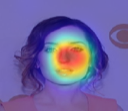
\includegraphics[height=\tableImHeight]{figures/chapter7/objSimilarity/faces/2/3_hm.png}} 
        \end{tabular}
    \caption{VGG-Faces}
    \end{subfigure}
    \begin{subfigure}[b]{\textwidth}
        \begin{tabular}{lc|cc|cc|cc}
        Whole Image &
        \raisebox{-.5\height}{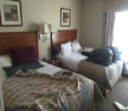
\includegraphics[height=\tableImHeight]{figures/chapter7/objSimilarity/traffickcam/orig/query.png}} & 
        \raisebox{-.5\height}{\fcolorbox{green}{green}{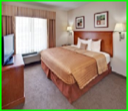
\includegraphics[height=\tableImHeight]{figures/chapter7/objSimilarity/traffickcam/orig/1_im.png}}} & 
        \raisebox{-.5\height}{\includegraphics[height=\tableImHeight]{figures/chapter7/objSimilarity/traffickcam/orig/1_hm.png}} & 
        \raisebox{-.5\height}{\fcolorbox{red}{red}{\includegraphics[height=\tableImHeight]{figures/chapter7/objSimilarity/traffickcam/orig/2_im.png}}} & 
        \raisebox{-.5\height}{\includegraphics[height=\tableImHeight]{figures/chapter7/objSimilarity/traffickcam/orig/2_hm.png}} & 
        \raisebox{-.5\height}{\fcolorbox{red}{red}{\includegraphics[height=\tableImHeight]{figures/chapter7/objSimilarity/traffickcam/orig/3_im.png}}} & 
        \raisebox{-.5\height}{\includegraphics[height=\tableImHeight]{figures/chapter7/objSimilarity/traffickcam/orig/3_hm.png}} 
        \\
        Region 1 &
        \raisebox{-.5\height}{\includegraphics[height=\tableImHeight]{figures/chapter7/objSimilarity/traffickcam/1/query.png}} & 
        \raisebox{-.5\height}{\fcolorbox{red}{red}{\includegraphics[height=\tableImHeight]{figures/chapter7/objSimilarity/traffickcam/1/1_im.png}}} & 
        \raisebox{-.5\height}{\includegraphics[height=\tableImHeight]{figures/chapter7/objSimilarity/traffickcam/1/1_hm.png}} & 
        \raisebox{-.5\height}{\fcolorbox{red}{red}{\includegraphics[height=\tableImHeight]{figures/chapter7/objSimilarity/traffickcam/1/2_im.png}}} & 
        \raisebox{-.5\height}{\includegraphics[height=\tableImHeight]{figures/chapter7/objSimilarity/traffickcam/1/2_hm.png}} & 
        \raisebox{-.5\height}{\fcolorbox{red}{red}{\includegraphics[height=\tableImHeight]{figures/chapter7/objSimilarity/traffickcam/1/3_im.png}}} & 
        \raisebox{-.5\height}{\includegraphics[height=\tableImHeight]{figures/chapter7/objSimilarity/traffickcam/1/3_hm.png}} 
        \\
        Region 2 &
        \raisebox{-.5\height}{\includegraphics[height=\tableImHeight]{figures/chapter7/objSimilarity/traffickcam/2/query.png}} & 
        \raisebox{-.5\height}{\fcolorbox{red}{red}{\includegraphics[height=\tableImHeight]{figures/chapter7/objSimilarity/traffickcam/2/1_im.png}}} & 
        \raisebox{-.5\height}{\includegraphics[height=\tableImHeight]{figures/chapter7/objSimilarity/traffickcam/2/1_hm.png}} & 
        \raisebox{-.5\height}{\fcolorbox{red}{red}{\includegraphics[height=\tableImHeight]{figures/chapter7/objSimilarity/traffickcam/2/2_im.png}}} & 
        \raisebox{-.5\height}{\includegraphics[height=\tableImHeight]{figures/chapter7/objSimilarity/traffickcam/2/2_hm.png}} & 
        \raisebox{-.5\height}{\fcolorbox{red}{red}{\includegraphics[height=\tableImHeight]{figures/chapter7/objSimilarity/traffickcam/2/3_im.png}}} & 
        \raisebox{-.5\height}{\includegraphics[height=\tableImHeight]{figures/chapter7/objSimilarity/traffickcam/2/3_hm.png}} 
        \end{tabular}
        \caption{TraffickCam}
    \end{subfigure}
    \caption{Object- and Region-Specific Retrieval. We show the most similar image from the three most similar classes when using either the whole image as the query input, or selected sub-regions of the image. This allows for object- or region- specific image retrieval; for example, ``find landmarks with similar archways'', ``find faces with brunette bangs'' or ``find hotels with similar looking bedspreads.'' }
    \label{fig:objSimilarity}
\end{figure*}
The previous experiments highlight the utility of the visualization method
on image retrieval tasks, which consider the entire image as input. The same visualization approach can also support object- or region-specific image retrieval.

We first compute the similarity maps between a query and the database images. Recall that the similarity map for a pair of images sums to the overall similarity score. Therefore, the sum of the values contained within subregions of the similarity map reflect the how much the subregion contributes to the match with the corresponding images. This subselection allows for database images to be sorted based on the contribution to the query image's similarity score at the region of interest. 
Figure~\ref{fig:objSimilarity} shows the most similar image from the three most similar classes for both whole image similarity and also using the highlighted sub-regions of the image. This modification allows for object- or region- specific image retrieval. For example, in the Google Landmarks dataset, searches can be constrained to find landmarks with similar archways or buildings with orange roofs. 

\todo{Incorporate experiments comparing image search w/ cropped objects as queries vs this approach.}